%%==========================================================================
\section{SuperMatching}
\label{sec:supersymhopm}
%-------------------------------------------------------------------------
We now discuss the first two issues mentioned above, which are independent of application; later we turn to sampling strategy and definition of affinity measure, which is application dependent.


\subsection{Supersymmetric Affinity Tensor}
\label{subsec:supersymtensor}

The supersymmetric higher-order affinity tensor is invariant under permutation of indices. The main motivation of using supersymmetry is to allow us to avoid redundant storage and computation.

\newtheorem{mot}{Definition}
\begin{mot}[Supersymmetric Tensor]
\label{mot:def1}
A tensor is  \emph{supersymmetric} if its entries are invariant under any permutation of its indices~\cite{Kofidis02}.
\end{mot}

For example, a third-order supersymmetric tensor $\mathcal{T}_3$, satisfies the relationships:
$\mathcal{T}_3(i_1, i_2, i_3)=\mathcal{T}_3(i_1, i_3, i_2)=\mathcal{T}_3(i_2, i_1, i_3)=\mathcal{T}_3(i_2, i_3, i_1)=\mathcal{T}_3(i_3, i_1, i_2)=\mathcal{T}_3(i_3, i_2, i_1)$.

\begin{mot}[Supersymmetric Affinity Tensor]
\label{mot:def2}
Given two feature sets $P_1$ and $P_2$, with $N_1$ and $N_2$ features respectively,
the supersymmetric affinity tensor is an $N^{th}$ order $I_1, \cdots, I_N$, nonnegative tensor $\mathcal{T}_N$,
for which there exists a set of indices $\theta_N$,
and an $N^{th}$ order potential function $\phi_N$, such that
%
\begin{flalign}
\mathcal{T}_N(i_1,\ldots,i_N) = \begin{cases}
\phi_N(\Omega(i_1,\ldots,i_N))&{,~\forall(i_1,\ldots,i_N)\in \theta_N}  \\
\quad{}\quad{}\quad{}   0     &{,~\forall(i_1,\ldots,i_N)\notin \theta_N}
\end{cases}
\end{flalign}
%
where $\Omega$ stands for an arbitrary permutation of the vector. $\theta_N$ satisfies $i_m \neq i_n$ $\forall (i_1,\ldots,i_N)\in \theta_N, \forall i_m\in\{i_1, \ldots, i_N\}$
and $\forall i_n\in\{i_1, \ldots, i_N\}-\{i_m\}$ .
\end{mot}

A tensor element with $(i_1,\ldots,i_N)\in \theta_N$ is called a \emph{potential element}, while other elements are called \emph{non-potential elements}.
A potential element represents one matching result out of all possible matching candidates.
Potential elements are further detailed in  Section~\ref{subsec:sampling}.

Using Definition~\ref{mot:def2}, we can reduce the amount of storage needed,  byrepresenting every potential element $\mathcal{T}_N(i_1,\ldots,i_N)$ by its canonical entry $\mathcal{T}_N(\mathrm{sort}(i_1,\ldots,i_N))$, $\forall (i_1,\ldots,i_N)\in \theta_N$. Each stored value thus provides the value for $N!$ entries.
Furthermore, as non-potential elements all have value zero, there is no need to store them.
This greatly reduces both storage, and the amount of feature tuple sampling
needed  when estimating the affinity tensor, as discussed in Section~\ref{subsec:sampling}.
At the same time, it can be used to make the power iteration process more efficient: see Section~\ref{subsec:oursymmhopm}.

%-------------------------------------------------------------------------
\subsection{Supersymmetric Higher-order Power Iteration}
\label{subsec:oursymmhopm}

\begin{algorithm}[!t]
\caption{\small Higher-order power iteration solution (with $\mathcal{C}_1$ norm) for the \protect\\
         \mbox{}\hspace{15ex}\small supersymmetric affinity tensor }
\label{alg2}
\begin{algorithmic}[1]
\REQUIRE \small $N{th}$-order supersymmetric affinity tensor
\ENSURE  \small Unit $\mathcal{\ell}^1$-norm vector $\boldsymbol{u}$
\STATE   \small \; Initialize $\boldsymbol{v}_0$ to random values in [0,1], $k=1$
\REPEAT
    \FOR{all $(i_1,\cdots , i_N)\in \theta_N$}
        \FOR{all $m \in (i_1,\cdots , i_N)$}
        \STATE $v_{m}^{(k)}=(N-1)!\phi_N(i_1,\cdots , i_N) 2v_{m}^{(k-1)}v_{i_1}^{2_{(k-1)}}\cdots$ \\
                 $\qquad \qquad v_{m-1}^{2_{(k-1)}}v_{m+1}^{2_{(k-1)}}\cdots v_{i_N}^{2_{(k-1)}}$
        \ENDFOR
        \FOR{$i=1:N_1$}
        \STATE $v^{(k)}(((i-1)\cdot N_2+1) : i\cdot N_2)=$   \protect\\
               $\hat{v}^{(k)}(((i-1)\cdot N_2+1) : i\cdot N_2)/\lVert \hat{v}^{(k)}(((i-1)\cdot N_2+1):i\cdot N_2)\lVert_1$
        \ENDFOR
    \ENDFOR
    \STATE $k=k+1$;
\UNTIL{\small convergence};
\STATE   \small \; $\boldsymbol{u}^{(k)}=\boldsymbol{v}^{2_{(k)}}$ \protect\\
       \small \textbf{Note}: $\boldsymbol{u}^{(k)}=\boldsymbol{v}^{2_{(k)}}$,
       \small and $v^{(k)}(((i-1)\cdot N_2+1) : i\cdot N_2)$ denotes the slice of $v^{(k)}$ with
       \small indices from $(i-1)\cdot N_2+1$ to $i\cdot N_2$.
\end{algorithmic}
\end{algorithm}

The higher-order tensor problem in Eq. (\ref{equ:assigment}) may be solved by tensor decomposition~\cite{Kolda08};
tensor decomposition originated in~\cite{Hitchcock27}.
We utilize the rank-one higher-order power method~\cite{Lathauwer95} to approximately solve Eq. (\ref{equ:assigment}); as noted, an exact computation is infeasible.
Eq. (\ref{equ:assigment}) can be expressed as:
\begin{eqnarray}
\label{equ:assigment2}
{\boldsymbol{x}}^* &=& \argmax_{\boldsymbol{x}} \sum_{i_1,i_2,\cdots,i_N} \mathcal{T}_N(i_1,\cdots,i_N) x_{i_1} \cdots x_{i_N} \nonumber\\
&=& \max <\mathcal{T}_N, \boldsymbol{x}^{\star N}>
\end{eqnarray}
where $\star$ is called the Tucker product~\cite{Kofidis02}, and $\boldsymbol{x} \in \{0,1\}^{N}$.
To get an approximate solution, we relax the constraints:
the binary assignment vector $\boldsymbol{x}\in \{0,1\}^{N}$ is replaced by an assignment vector $\boldsymbol{u}$ with elements taking real values in $[0,1]$.
This changes the optimization problem to one of computing the rank-one approximation of the affinity tensor $\mathcal{T}_N$~\cite{Kofidis02},
i.e.\ finding a scalar $\lambda$ and a unit norm vector $\boldsymbol{u}\in \mathbb{R}^{N}$,
such that the tensor $\hat{\mathcal{T}_N} = \lambda \boldsymbol{u}\star \boldsymbol{u} \star\cdots \star \boldsymbol{u}=\boldsymbol{u}^{\star N}$ minimizes the Frobenius norm squared function $f(\hat{\mathcal{T}_N})=\lVert \mathcal{T}_r-\hat{\mathcal{T}_N} \lVert^2_F$.
The final matching result is found by replacing each element of $\boldsymbol{u}$ by 0 or 1 according to whichever it is closer to.

The higher-order power method is commonly used for finding rank-one tensor approximations; a version for supersymmetric tensors (S-HOPM) is given in~\cite{Kofidis02}.
The S-HOPM algorithm converges under the assumption of convexity (or concavity) for the functional induced by the tensor~\cite{Kofidis02},
which is sufficiently robust for practical applications.
S-HOPM is performed in two iterative steps: higher-order power iteration of $\boldsymbol{u}$, followed by normalization of $\boldsymbol{u}$ under the Frobenius norm.
A recent effective improvement~\cite{Duchenne09} uses the $\mathcal{\ell}^1$ norm to replace the traditional $\mathcal{\ell}^2$ norm.


We both use the $\mathcal{\ell}^1$ norm, and further revise S-HOPM as follows.
To perform higher-order power iteration of $\boldsymbol{u}$, we must compute $\hat{\boldsymbol{u}}^{(k)}=\mathcal{I}\mathop{\star}\limits^{\mathcal{T}_N}
{(\boldsymbol{u}^{(k-1)})}^{\mathop{\star}\limits^{\mathcal{T}_N} (N-1)}$, where
$\mathop{\star}\limits^{\mathcal{T}_N}$ is a so-called $\mathcal{T}_N$-product,
and $\mathcal{I}$ is the unit tensor~\cite{Kofidis02}.
For $\hat{\boldsymbol{u}}^{(k)}$ belonging to an $N{th}$-order supersymmetric affinity tensor, this can be formulated as follows:
%\begin{small}
\begin{flalign}
\label{equ:eqsmain2}
&\hat{\boldsymbol{u}}^{(k)}=\mathcal{I}\mathop{\star}\limits^{\mathcal{T}_N}
{(\boldsymbol{u}^{(k-1)})}^{\mathop{\star}\limits^{\mathcal{T}_N} (N-1)} \mathrm{~implies~that~} \forall m\in (i_1,... , i_N), \nonumber \\
&v_{m}^{(k)} = \nonumber\\
&\sum\limits_{i_1,...,i_N}\mathcal{T}_N(i_1,...,i_N)2v_{m}^{(k-1)}v_{i_1}^{2_{(k-1)}}... v_{m-1}^{2_{(k-1)}}v_{m+1}^{2_{(k-1)}}... v_{i_N}^{2_{(k-1)}}= \nonumber \\
&(N-1)!\phi_N(i_1,...,i_N)2v_{m}^{(k-1)}v_{i_1}^{2_{(k-1)}}... v_{m-1}^{2_{(k-1)}}v_{m+1}^{2_{(k-1)}}... v_{i_N}^{2_{(k-1)}}
\end{flalign}
%\end{small}
where $\boldsymbol{u}^{(k)}=\boldsymbol{v}^{2_{(k)}}$, and $\phi_N$ is the  potential function explained in Section~\ref{subsec:potentials}.
Eq. (\ref{equ:eqsmain2}) is more compact than earlier expressions in the literature, as it handles all symmetrically related potential elements as a single item using   multiplication by $(N-1)!$.

Many initialization schemes have been proposed for the S-HOPM method~\cite{Kofidis02}.
We simply use positive random values between $0$ and $1$ to initialize $\boldsymbol{u}_0$, which ensures convergence; proofs are detailed in~\cite{Regalia00,Kofidis02}.

Our supersymmetric higher-order power iteration solution of Eq. (\ref{equ:assigment}) is performed by the SuperMatching algorithm---see Algorithm~\ref{alg2}. Its efficiency relies on two principles.
First, we take advantage of the supersymmetry to deduce $\boldsymbol{u}$ as in Eq. (\ref{equ:eqsmain2}), using just a single canonical element for computation (see Step 5).
Secondly, power iteration just consides the non-zero potential elements, and excludes each non-potential element from the iteration process.
The complexity of the whole iteration process  depends only on the number $|\theta_N|$ of non-zero affinities.
Consequently, this method reduces also memory costs while keeping accuracy.

Note that, although~\cite{Duchenne09} claimed to use a supersymmetric affinity tensor,
his approach does not make full use of supersymmetry when creating the supersymmetric affinity tensor,
nor does it take advantage of supersymmetry to accelerate the power iteration process.
By doing so, we overcome limitations due to unbalanced and redundant tensor elements in~\cite{Duchenne09}, as our experiments show later.



%-------------------------------------------------------------------------
\subsection{Sampling Strategy}
\label{subsec:sampling}

Algorithm~\ref{alg2} depends on the potential elements.
We next discuss the issue of how to sample the feature tuples to build potential items, which determines the size $|\theta_N|$ and influences matching accuracy (and speed).

Given the two feature sets $P_1$ and $P_2$,
a potential element may be obtained by using a feature tuple sampled from each feature set separately.
For $N^{th}$-order matching, a naive way to construct the potential elements is as follows:
first find all feature tuples for $P_1$ and $P_2$, as $F_1$ and $F_2$; then $\forall (f_{i_1}^1, \cdots, f_{i_N}^1)\in F_1$,
calculate the potentials for $(f_{i_1}^1, \cdots, f_{i_N}^1)$ with all feature tuples in $F_2$.
This is far too time-consuming, so sampling is used instead.
We suggest random sampling for general feature matching problems,
but this does not preclude more directed sampling if prior knowledge of the matching problems gives guidance.

Our sampling approach is to repeatedly randomly sample $t_1$ feature tuples for each feature point from $P_1$, and fully sample $P_2$.
For $P_1$, we take each feature in turn as a required element, and then randomly choose $t_1$ feature tuples containing this required element.
Thus, the number of feature tuples in $F_1$ is $N_1t_1$, and $N_2^N$ in $F_2$.
Then, for each feature tuple in $F_1$, we find the $k$ most similar features in $F_2$ to build $k$ potential elements as $\phi_i^k$.
Combining all the potential elements obtained, we form the desired potential element set $\theta_N = \{\phi_i^k\}_{i=1}^{N_1 t_1}$, of size $|\theta_N| = N_1 t_1 k$.
For $P_1$, the sampling cost is $O(N_1  t_1 k \log N_2)$, where the $\log N_2$ arises from use of a $k$D-tree to search for the $k$ most similar features in $F_2$.
The parameters $t_1$ and $k$ must be chosen according to the size of the feature sets.
In practice, for two feature sets each with hundreds points,
we may take $t_1 \approx 100$ and $k\approx300$ for third-order matching.
Our experiments demonstrate that this sampling approach works well.

An important aspect of our sampling approach is to use the supersymmetry of the affinity tensor. Potential elements whose indices are permutations of each other
have the same value, so should not be repeatedly sampled.
Thus, we use a sampling constraint that the sets of feature tuples $F_1$ obtained from the sampling process should have no repetition, in the sense that
\begin{eqnarray}
\label{equ:noredun2}
\forall (f_{i_1}^1,f_{i_2}^1,\cdots,f_{i_N}^1),(f_{j_1}^1,f_{j_2}^1,\cdots,f_{j_N}^1) \in F_1,\nonumber\\ (f_{i_1}^1,f_{i_2}^1,\cdots,f_{i_N}^1)\neq\Omega(f_{j_1}^1,f_{j_2}^1,\cdots,f_{j_N}^1)
\end{eqnarray}
where $\Omega$ is an arbitrary permutation.

Earlier work~\cite{Zass08,Duchenne09,Aiping10} adopted random sampling,
but failed to impose any constraint on the sampling process to take into account supersymmetry,
leading to the possibility that feature tuples may be sampled multiple times.
For example, for third-order matching, it is possible that a feature tuple $(f_{i_1}^1, f_{i_2}^1, f_{i_3}^1)$ may be sampled from $P_1$ and $(f_{i_1}^2, f_{i_2}^2, f_{i_3}^2)$ from $P_2$,
and also a feature tuple $(f_{i_1}^1, f_{i_3}^1, f_{i_2}^1)$  from $P_1$ and $(f_{i_1}^2, f_{i_3}^2, f_{i_2}^2)$ from $P_2$. That would create two tensor elements $\phi_3({i_1}, {i_2}, {i_3})$ with index $({i_1}, {i_2}, {i_3})$ and $\phi_3({i_1}, {i_3}, {i_2})$ with index $({i_1}, {i_3}, {i_2})$, which are the same. However, we just need one tensor element to express the affinity on the assignment group $({i_1}, {i_2}, {i_3})$ for any permutation of indices.
This extra sampling is not only inefficient, but may also reduce the accuracy of the power iteration: one set of symmetrically related elements  may be represented by a different number of samples than another set of  symmetrically related elements, which unbalances the power iteration process, and can lead to inaccurate results.
Our sampling method reduces the sampling cost, while also improving the accuracy of the power iteration.

\subsection{Higher-order Potentials}
\label{subsec:potentials}

Different higher-order potentials are appropriate for different applications.
Here we briefly give two simple examples of general higher-order potentials for  2D and 3D matching respectively; we  use them later to evaluate our algorithm.
The potentials are based on a Gaussian function
which guarantees the tensor elements are non-negative and invariant under any permutation of the input assignments.

In 2D, we use a well-known third-order geometric-similarity invariant potential $\phi_3$~\cite{Duchenne09,Chertok10} for linking point feature triples.
Triangles formed by three points are \emph{similar} under scaling, rotation and translation---interior angles are invariant.
Thus $\phi_3$ can be defined in terms of differences of corresponding interior angles:
\begin{eqnarray}
\phi_3(i_1,i_2,i_3)&=&\phi_3(\{p_1,q_1\}, \{p_2,q_2\}, \{p_3,q_3\})\nonumber\\
&=&\exp(-1/\varepsilon^2\sum\nolimits_{(l,l^{'})}\lVert \alpha_l- \alpha_{l^{'} } \lVert^2 )
\end{eqnarray}
where $\varepsilon > 0$ is the kernel bandwidth, which is automatically determined as the average of the $\mathcal{\ell}^1$ norm of all differences,
and $\{\alpha_l\}_{l=1}^3$ and $\{\alpha_l^{'}\}_{l^{'}=1^{'}}^{3}$ are the angles formed by feature triples $(p_1,p_2,p_3)$ and $(q_1,q_2,q_3)$:
see Figure~\ref{fig:TO}. Each point corresponds to one interior angle.
We may extend it to higher order by using the internal angles formed by polygons with more than 3 sides.

For 3D matching problems, we may replace the internal angles by edge lengths, which for meshes are based on geodesic distance across the mesh in which the points are embedded. This corresponds to assuming an isometry transform relating the meshes.
Geodesic distance may be computed by Dijkstra's algorithm~\cite{Peyre2010}.
See  Figure~\ref{fig:TO}.

\begin{figure}
\centering
  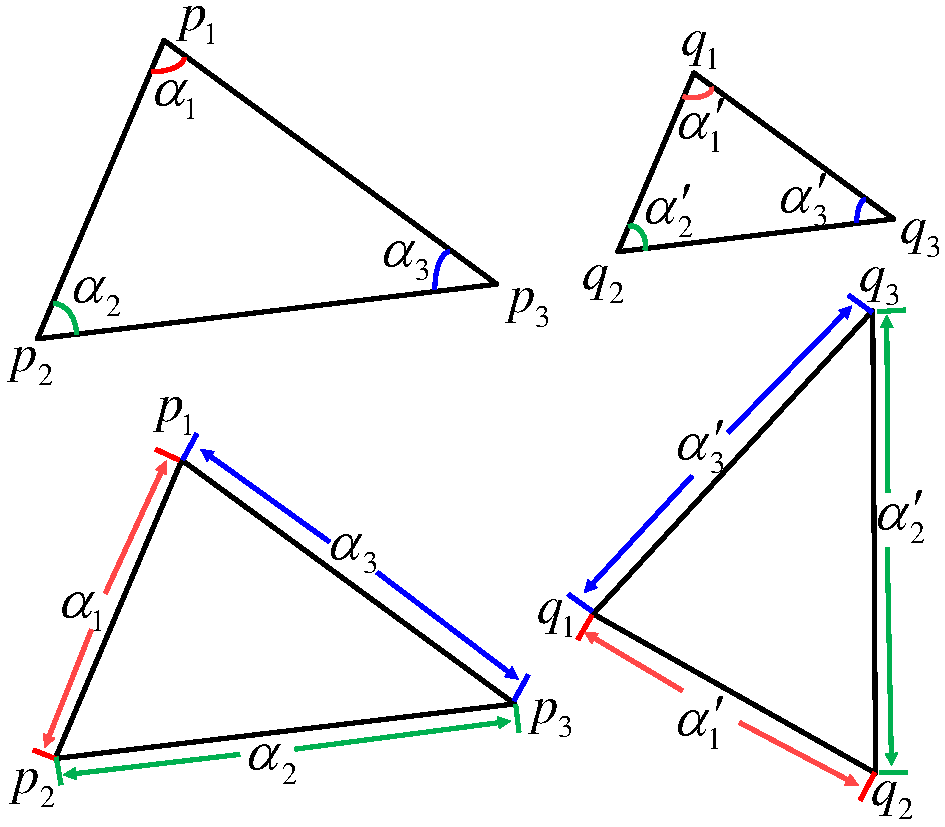
\includegraphics[width=0.6\linewidth]{figures/diagram.pdf}
  \caption{Third-order potential. The geometric constraints are: internal angle invariance in 2D (above), and edge length invariance in 3D (below).}
\label{fig:TO}
\end{figure}

